\documentclass{article}

%\usepackage[utf8]{inputenc}		% LuaTex do not need this
%\usepackage[T1]{fontenc}			% LuaTex do not need this
\usepackage{fontspec}				% LuaTex need this
\usepackage{lmodern}
\usepackage{comment}
\usepackage[a4paper]{geometry}
\usepackage{graphicx}
	\graphicspath{ {Bilder/} }

%%%%%%%%%%%%%%%%%%%%%%%%%%%%%%%%%%%%%%%%%%%%%%%%%%%%%%%%%%%%%%%%%%%%%%%%%%%%%%%%
%
% https://tex.stackexchange.com/questions/82993/how-to-change-the-name-of-document-elements-like-figure-contents-bibliogr
% https://tex.stackexchange.com/questions/186946/changing-the-autoref-name-for-chapter
%
%\usepackage[ngerman]{babel}		% LuaTex do not need this
\usepackage{polyglossia}
	\setdefaultlanguage[spelling=new]{german}
	\addto\captionsgerman{
		\renewcommand{\figurename}{Abbildung}
		\renewcommand{\figureautorefname}{Abbildung}
		\renewcommand{\equationautorefname}{Gleichung}
	}


%%%%%%%%%%%%%%%%%%%%%%%%%%%%%%%%%%%%%%%%%%%%%%%%%%%%%%%%%%%%%%%%%%%%%%%%%%%%%%%%
%
% LATEX Mathematical Symbols
% https://reu.dimacs.rutgers.edu/Symbols.pdf
% https://en.wikibooks.org/wiki/LaTeX/Mathematics
%
\usepackage{amssymb}
\usepackage{amsthm}
\usepackage{amsmath}

%%%%%%%%%%%%%%%%%%%%%%%%%%%%%%%%%%%%%%%%%%%%%%%%%%%%%%%%%%%%%%%%%%%%%%%%%%%%%%%%
%
% algorithm2e.sty — package for algorithms
% http://ctan.mirrors.hoobly.com/macros/latex/contrib/algorithm2e/doc/algorithm2e.pdf
%
\usepackage[
	ngerman,
	linesnumbered,
	boxed,
%	algochapter,
%	rightnl,
%	figure,
]{algorithm2e}
	% Then you can adjust the spacing between the body of the algorithm and its
	% caption through the command \SetAlCapSkip.
	\SetAlCapSkip{1em}
	% Restyling the caption in an algorithm created with algorithm2e
	% https://tex.stackexchange.com/questions/112294/restyling-the-caption-in-an-algorithm-created-with-algorithm2e/112295
	\SetAlgoCaptionSeparator{:}
	\renewcommand\AlCapFnt{\normalfont}
	% Algorithm2e modify line numbers
	% https://tex.stackexchange.com/questions/100145/algorithm2e-modify-line-numbers
	\SetNlSty{textbf}{}{:}
	% Sets the value of the space between the line numbers and the text, by default 1em.
	\SetNlSkip{2em}
	%\SetAlgoRefName{QXY}

%%%%%%%%%%%%%%%%%%%%%%%%%%%%%%%%%%%%%%%%%%%%%%%%%%%%%%%%%%%%%%%%%%%%%%%%%%%%%%%%
%
% TikZ
%
\usepackage{tikz}
	\usetikzlibrary{arrows.meta,graphs,shapes,trees}
\usepackage{tkz-berge}
\usepackage{tkz-graph}
\makeatletter
\pgfmathdeclarefunction{alpha}{1}{%
	\pgfmathint@{#1}%
	\edef\pgfmathresult{\pgffor@alpha{\pgfmathresult}}%
}
%%%%%%%%%%%%%%%%%%%%%%%%%%%%%%%%%%%%%%%%%%%%%%%%%%%%%%%%%%%%%%%%%%%%%%%%%%%%%%%%
%
% https://www.dante.de/events/Archiv/dante2012/Programm/Vortraege/vortrag-ferber.pdf
%
\usepackage[
	breaklinks,
	colorlinks,
	linkcolor=black,
	urlcolor=black,
	citecolor=black,
	pdfencoding=auto,
	ngerman
]{hyperref}
%%%%%%%%%%%%%%%%%%%%%%%%%%%%%%%%%%%%%%%%%%%%%%%%%%%%%%%%%%%%%%%%%%%%%%%%%%%%%%%%
%
%
%
\usepackage{verbatim}
\usepackage{float}
\usepackage{subcaption}
	\captionsetup{subrefformat=parens}
\usepackage{rail}
	\railalias{exp}{<Exp>}
	\railalias{stmt}{<Stmt>}
\usepackage{tabto}

%
% Längenangabe für die Einrückung der ersten Zeile eines neuen Absatzes.	
% https://golatex.de/wiki/%5Cparindent
%
\setlength{\parindent}{0mm}


%%%%%%%%%%%%%%%%%%%%%%%%%%%%%%%%%%%%%%%%%%%%%%%%%%%%%%%%%%%%%%%%%%%%%%%%%%%%%%%%
%
%
%
\title{Technische Informatik\\ Lösungen zu der Übung 5}

\author{
	Albert Kasdorf\and
	Georg Braun
}
\date{22.05.2018}



%%%%%%%%%%%%%%%%%%%%%%%%%%%%%%%%%%%%%%%%%%%%%%%%%%%%%%%%%%%%%%%%%%%%%%%%%%%%%%%%
%
%
%
\begin{document}

\maketitle

\section*{Aufgabe 39 (CFGs)}
Betrachten Sie die CFG GSE in \autoref{fig:compilerbau_abbildung_11_18} und das Wort

\begin{equation*}
	\text{w = IDENT "=" NUMBER "*" IDENT "*" NUMBER ";".}
\end{equation*}

\begin{figure}[h]
	\centering
	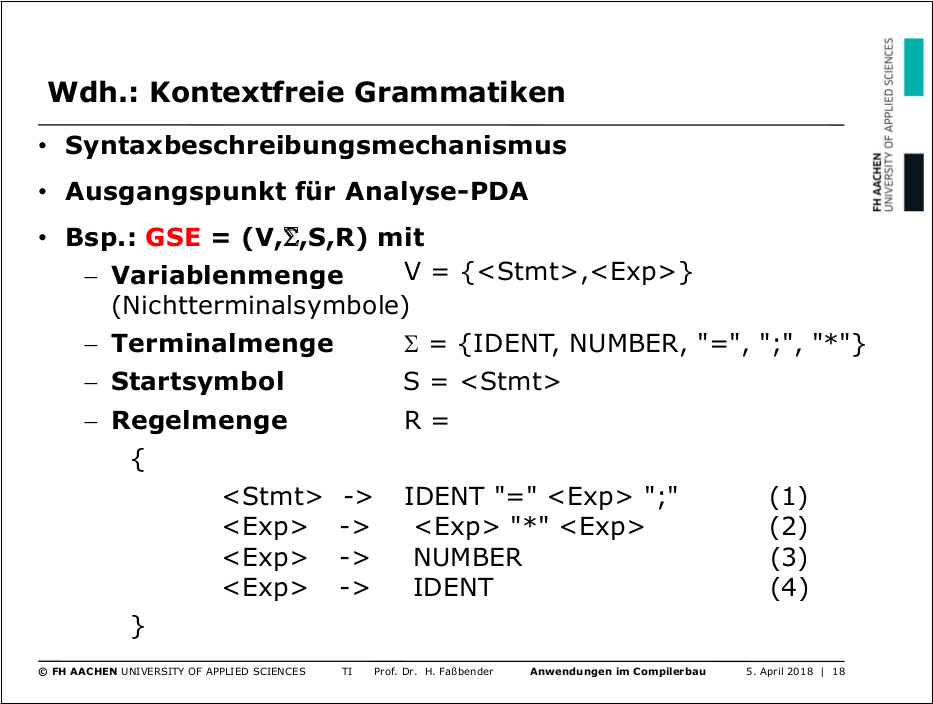
\includegraphics[width=0.75\linewidth]{Compilerbau_Abbildung_11_18}
	\caption{Wdh.: Kontextfreie Grammatiken}
	\label{fig:compilerbau_abbildung_11_18}
\end{figure}

\newpage
\subsection*{a) Geben Sie ein Syntaxdiagramm an, das die durch GSE erzeugte Sprache beschreibt.}

\begin{rail}
	stmt : 'IDENT' '=' exp ';'
\end{rail}

\begin{rail}
	exp : exp '*' exp | 'NUMBER' | 'IDENT'
\end{rail}

\begin{center}
%	\begin{tabular}{|l|r|c|l|r|l|c|}
	\begin{tabular}{lrclrlc}
		& GSE & = & \multicolumn{4}{l}{(V, $\Sigma$, S, R)} \\
		Variablenmenge & V & = & \multicolumn{4}{l}{\{<Stmt>, <Exp>\}} \\
		Terminalmenge & $\Sigma$ & = & \multicolumn{4}{l}{\{IDENT, NUMBER, "=", ";", "*"\}} \\
		Startsymbol & S & = & \multicolumn{4}{l}{\{<Stmt>\}} \\
		Regelmenge & R & = & \{ \\
		& & & & <Stmt> & $\rightarrow$ IDENT "=" <Exp> ";" & (1) \\
		& & & & <Exp> & $\rightarrow$ <Exp> "*" <Exp> & (2) \\
		& & & & <Exp> & $\rightarrow$ NUMBER & (3) \\
		& & & & <Exp> & $\rightarrow$ IDENT & (4) \\
		& & & \} \\
		\\
		& w & = & \multicolumn{4}{l}{IDENT "=" NUMBER "*" IDENT "*" NUMBER ";"}
	\end{tabular}
\end{center}

\subsection*{b) Geben Sie eine Linksableitung von w an.}

\begin{center}
	\begin{tabular}{rll}
		<Stmt> & & Regel \\
		=l> & IDENT "=" <Exp> ";" & (1) \\
		=l> & IDENT "=" <Exp> "*" <Exp> ";" & (2)\\
		=l> & IDENT "=" NUMBER "*" <Exp> ";" & (3)\\
		=l> & IDENT "=" NUMBER "*" <Exp> "*" <Exp> ";" & (2)\\
		=l> & IDENT "=" NUMBER "*" IDENT "*" <Exp> ";" & (4)\\
		=l> & IDENT "=" NUMBER "*" IDENT "*" NUMBER ";" & (3)\\
	\end{tabular}
\end{center}

\subsection*{c) Geben Sie eine Rechtsableitung von w an.}

\begin{center}
	\begin{tabular}{rll}
		<Stmt> & & Regel \\
		=r> & IDENT "=" <Exp> ";" & (1) \\
		=r> & IDENT "=" <Exp> "*" <Exp> ";" & (2)\\
		=r> & IDENT "=" <Exp> "*" NUMBER ";" & (3)\\
		=r> & IDENT "=" <Exp> "*" <Exp> "*" NUMBER ";" & (2)\\
		=r> & IDENT "=" <Exp> "*" IDENT "*" NUMBER ";" & (4)\\
		=r> & IDENT "=" NUMBER "*" IDENT "*" NUMBER ";" & (3)\\
	\end{tabular}
\end{center}


\section*{Aufgabe 40 (Mehrdeutige CFGs)}

\subsection*{a) Geben Sie eine CFG und ein Wort w an, so dass es für das Wort w zwei verschiedene Linksableitungen zu w gibt und beweisen Sie Ihre Aussage durch Angabe der beiden Linksableitungen zu w.}

\begin{center}
	%	\begin{tabular}{|l|r|c|l|r|l|c|}
	\begin{tabular}{lrclrlc}
		& GSE & = & \multicolumn{4}{l}{(V, $\Sigma$, S, R)} \\
		Variablenmenge & V & = & \multicolumn{4}{l}{\{<Stmt>, <Exp>\}} \\
		Terminalmenge & $\Sigma$ & = & \multicolumn{4}{l}{\{IDENT, NUMBER, "=", ";", "*"\}} \\
		Startsymbol & S & = & \multicolumn{4}{l}{\{<Stmt>\}} \\
		Regelmenge & R & = & \{ \\
		& & & & <Stmt> & $\rightarrow$ IDENT "=" <Exp> ";" & (1) \\
		& & & & <Exp> & $\rightarrow$ <Exp> "*" <Exp> & (2) \\
		& & & & <Exp> & $\rightarrow$ NUMBER & (3) \\
		& & & & <Exp> & $\rightarrow$ IDENT & (4) \\
		& & & \} \\
		\\
		& w & = & \multicolumn{4}{l}{IDENT "=" NUMBER "*" IDENT "*" NUMBER ";"}
	\end{tabular}
\end{center}

\subsection*{b) Zeichnen Sie zu jeder Linksableitung den zugehörigen Syntaxbaum.}

\begin{figure}[H]
	\centering
	\subcaptionbox{Regel: 123234}[.49\linewidth]
	{
		\begin{tikzpicture}[scale=0.90]
		\node{<Stmt>}
		child{node{IDENT}}
		child{node{"="}}
		child{node{<Exp>}
			child{node{<Exp>}
				child{node{NUMBER}}
				child[missing]
			}
			child{node{"*"}}
			child{node{<Exp>}
				child{node{<Exp>}
					child{node{IDENT}}
				}
				child{node{"*"}}
				child{node{<Exp>}
					child{node{NUMBER}}
				}
			}
		}
		child{node{";"}}
		;
		\end{tikzpicture}
	}
	\hfill
	\subcaptionbox{Regel: 122343}[.49\linewidth]
	{
		\begin{tikzpicture}[scale=0.90]
		\node{<Stmt>}
		child{node{IDENT}}
		child{node{"="}}
		child{node{<Exp>}
			child{node{<Exp>}
				child{node{<Exp>}
					child{node{NUMBER}}
				}
				child{node{"*"}}
				child{node{<Exp>}
					child{node{IDENT}}
				}
			}
			child{node{"*"}}
			child{node{<Exp>}
				child[missing]
				child{node{NUMBER}}
			}
		}
		child{node{";"}}
		;
		\end{tikzpicture}
	}
\end{figure}


\newpage
\section*{Aufgabe 41 (CNF)}

Geben Sie eine Typ 2-Grammatik an, die die folgende Sprache erzeugt und transformieren Sie diese in CNF: $\{a^n b^n c^n \mid n,m \ge 1\}$.

Typ 2-Grammatik:
$G = (\{S, C, D\}, \{a, b, c\}, S, P)$ mit
\begin{equation}
\begin{split}
P = \{ \\\
&S \rightarrow CD, \\\
&C \rightarrow aCb, \\\
&C \rightarrow ab, \\\
&D \rightarrow cD, \\\
&D \rightarrow c \}
\end{split}
\end{equation}

Nun die Umformung in CNF:
Für die Umformung die nicht alleinstehende Terminale in Variablen überführen. Werden mehr als zwei Nichtterminale auf der rechten Regelseite vorkommen werden diese durch eine neue Variable ersetzt.

Typ 2-Grammatik in CNF:
$G = (\{S, C, X, D, V_a, V_b, V_c\}, \{a, b, c\}, S, P)$ mit
\begin{equation}
\begin{split}
P = \{ \\\
&S \rightarrow CD, \\
&C \rightarrow XV_b, \\\
&X \rightarrow V_aC, \\\
&C \rightarrow V_aV_b, \\\
&D \rightarrow V_cD, \\\
&D \rightarrow c, \\\
&V_a \rightarrow a, \\\
&V_b \rightarrow b, \\\
&V_c \rightarrow c \} \\\
\end{split}
\end{equation}


\newpage
\section*{Aufgabe 42 (Top-Down-Analyserechnung)}

\subsection*{a) Geben Sie eine CFG an, die die Menge der nichtleeren Palindrome (Wort gleich dem gespiegelten Wort) über dem Alphabet $\Sigma = \left\{a, b, c\right\}$ erzeugt. Bsp.: $w=abccba$ ist in der zu erzeugenden Menge.}

$G = (\{S\}, \{a, b, c\}, S, P)$ mit
\begin{equation}
\begin{split}
P = \{ \\\
&\quad (1) \quad S \rightarrow aSa, \\\ 
&\quad (2) \quad S \rightarrow bSb, \\\
&\quad (3) \quad S \rightarrow cSc, \\\
&\quad (4) \quad S \rightarrow aa, \\\
&\quad (5) \quad S \rightarrow bb, \\\
&\quad (6) \quad S \rightarrow cc, \\\
&\quad (7) \quad S \rightarrow a, \\\
&\quad (8) \quad S \rightarrow b, \\\
&\quad (9) \quad S \rightarrow c \} \\\
\end{split}
\end{equation}

\subsection*{b) Geben Sie eine Top-Down Analyserechnung des Top-Down Analyseautomaten zur CFG aus Teil a) für das Wort $w=abccba$ an, die erfolgreich ist.}

\begin{equation}
\begin{split}
&\Rightarrow(z, abccba, S, ) \\\ 
&\Rightarrow(z, abccba, aSa, 1) \\\ 
&\Rightarrow(z, bccba, Sa, 1) \\\ 
&\Rightarrow(z, bccba, bSba, 1 2) \\\ 
&\Rightarrow(z, ccba, Sba, 1 2) \\\
&\Rightarrow(z, ccba, ccba, 1 2 6) \\\
&\Rightarrow(z, cba, cba, 1 2 6) \\\
&\Rightarrow(z, ba, ba, 1 2 6) \\\
&\Rightarrow(z, a, a, 1 2 6) \\\
&\Rightarrow(z, , , 1 2 6) \\\
\end{split}
\end{equation}


\subsection*{c) Geben Sie eine Top-Down Analyserechnung des Top-Down Analyseautomaten zur CFG aus Teil a) für das Wort $w=abccba$ an, die erfolglos abbricht.}

\begin{equation}
\begin{split}
&\Rightarrow(z, abccba, S, ) \\\ 
&\Rightarrow(z, abccba, S, 9) \\\ 
&\Rightarrow(z, abccba, c, 9) \\\ 
&c \neq a
\end{split}
\end{equation}

\newpage
\section*{Aufgabe 43 (Durchschnitt Typ 2-Sprachen)}

\subsection*{a) Beweisen oder widerlegen Sie, dass der Schnitt von $L_1$ und $L_2$, aus Aufgabe 37 und 38, vom Typ 2 ist.}

\begin{align}
	L_1 &= \{a^n b^n c^m \mid n, m > 0\} \nonumber\\
	L_2 &= \{a^n b^m c^m \mid n, m > 0\} \nonumber
\end{align}

\begin{table}[H]
	\centering
	\begin{tabular}{|c|c|c|c|c|c|c|c|c|}
		\hline
		$n,m$ & $1,1$ & $1,2$ & $2,1$ & $2,2$ & $2,3$ & $3,2$ & $3,3$ & $\cdots$ \\
		\hline
		$L_1$ & abc & ab\,cc & aabb\,c & aabbcc & aabb\,ccc & aaabbb\,cc & aaabbbccc & $\cdots$ \\
		%\hline
		$L_2$ & abc & a\,bbcc & aa\,bc & aabbcc & aa\,bbbccc & aaa\,bbcc & aaabbbccc & $\cdots$ \\
		\hline
	\end{tabular}
	\caption{Bildung einiger Wörter mit der Sprache $L_1$ und $L_2$.}
	\label{tab:some_words_of_language_one_and_two}
\end{table}

Beweis durch Angabe eines Gegenbeispiels: Aus der \autoref{tab:some_words_of_language_one_and_two} kann entnommen werden, dass beide Sprachen die selben Wörter erzeugen, wenn $n=m$ gilt. Somit ergibt sich aus dem Schnitt der beiden Sprachen die folgende Sprache:

\begin{align}
L_1 \cap L_2 &= \{a^n b^n c^n \mid n > 0\} \nonumber
\end{align}

Mit Hilfe des Pumping Lemmas kann nachgewiesen werden, dass der Schnitt nicht mehr vom Typ 2 ist.

\subsection*{b) Was bedeutet das für die Abschlusseigenschaften der Typ 2-Sprachen?}

Der Schnitt zweier Typ 2-Sprachen ist also nicht zwingend wieder vom Typ 2.


\newpage
\section*{Aufgabe 44 (Typ 1-Sprache)}

\subsection*{Zeigen Sie, dass die Sprache $L = \left\{a^m b^m c^m \mid m \geq 1\right\}$ vom Typ 1 ist.}

Ziel: Eine Grammatik von Typ 1 finden.
$G = (\{S\}, \{a, b, c\}, S, P)$ mit
\begin{equation}
\begin{split}
P = \{ \\\
&\quad (1) \quad S \rightarrow aSBC, \quad \text{; weitere Verschachtelung} \\\ 
&\quad (2) \quad S \rightarrow aBC, \quad \text{;Ende der Generierung} \\\
&\quad (3) \quad CB \rightarrow BC, \quad \text{;Variablen wieder in Reihenfolge bringen} \\\
&\quad (4) \quad aB \rightarrow ab, \quad \text{;Übergung von a zu B} \\\
&\quad (5) \quad bB \rightarrow bb, \quad \text{; Anpassung im B Bereich} \\\
&\quad (6) \quad bC \rightarrow bc, \quad \text{; Übergang von b zu C} \\\
&\quad (7) \quad cC \rightarrow cc \} \quad \text{; Anpassung im C Bereich} \\\
\end{split}
\end{equation}

Ein Beispiel für das Wort $w=aaabbbccc$
\begin{equation}
\begin{split}
&S \Rightarrow_1 aSBC \\\ 
&\Rightarrow_1 aaSBCBC \\\ 
&\Rightarrow_2 aaaBCBCBC \\\ 
&\Rightarrow_3 aaaBBCCBC \\\ 
&\Rightarrow_3 aaaBBCBCC \\\ 
&\Rightarrow_3 aaaBBBCCC \\\ 
&\Rightarrow_4 aaabBBCCC \\\ 
&\Rightarrow_5 aaabbBCCC \\\
&\Rightarrow_5 aaabbbCCC \\\ 
&\Rightarrow_6 aaabbbcCC \\\ 
&\Rightarrow_7 aaabbbccC \\\ 
&\Rightarrow_7 aaabbbccc \\\ 
\end{split}
\end{equation}


\end{document}